\section{Managing Exhibitions}\label{sec:managing-exhibitions}
The \emph{Manage exhibitions} page is similar to the \emph{Manage artists} page. Here, the list of exhibitions is presented. Every exhibition can
be edited or deleted, similar to the artist list. Each entry shows where and when the exhibition took place, together with the list of artists
that attended the exhibition.

\begin{figure}[hbt!]
    \begin{center}
        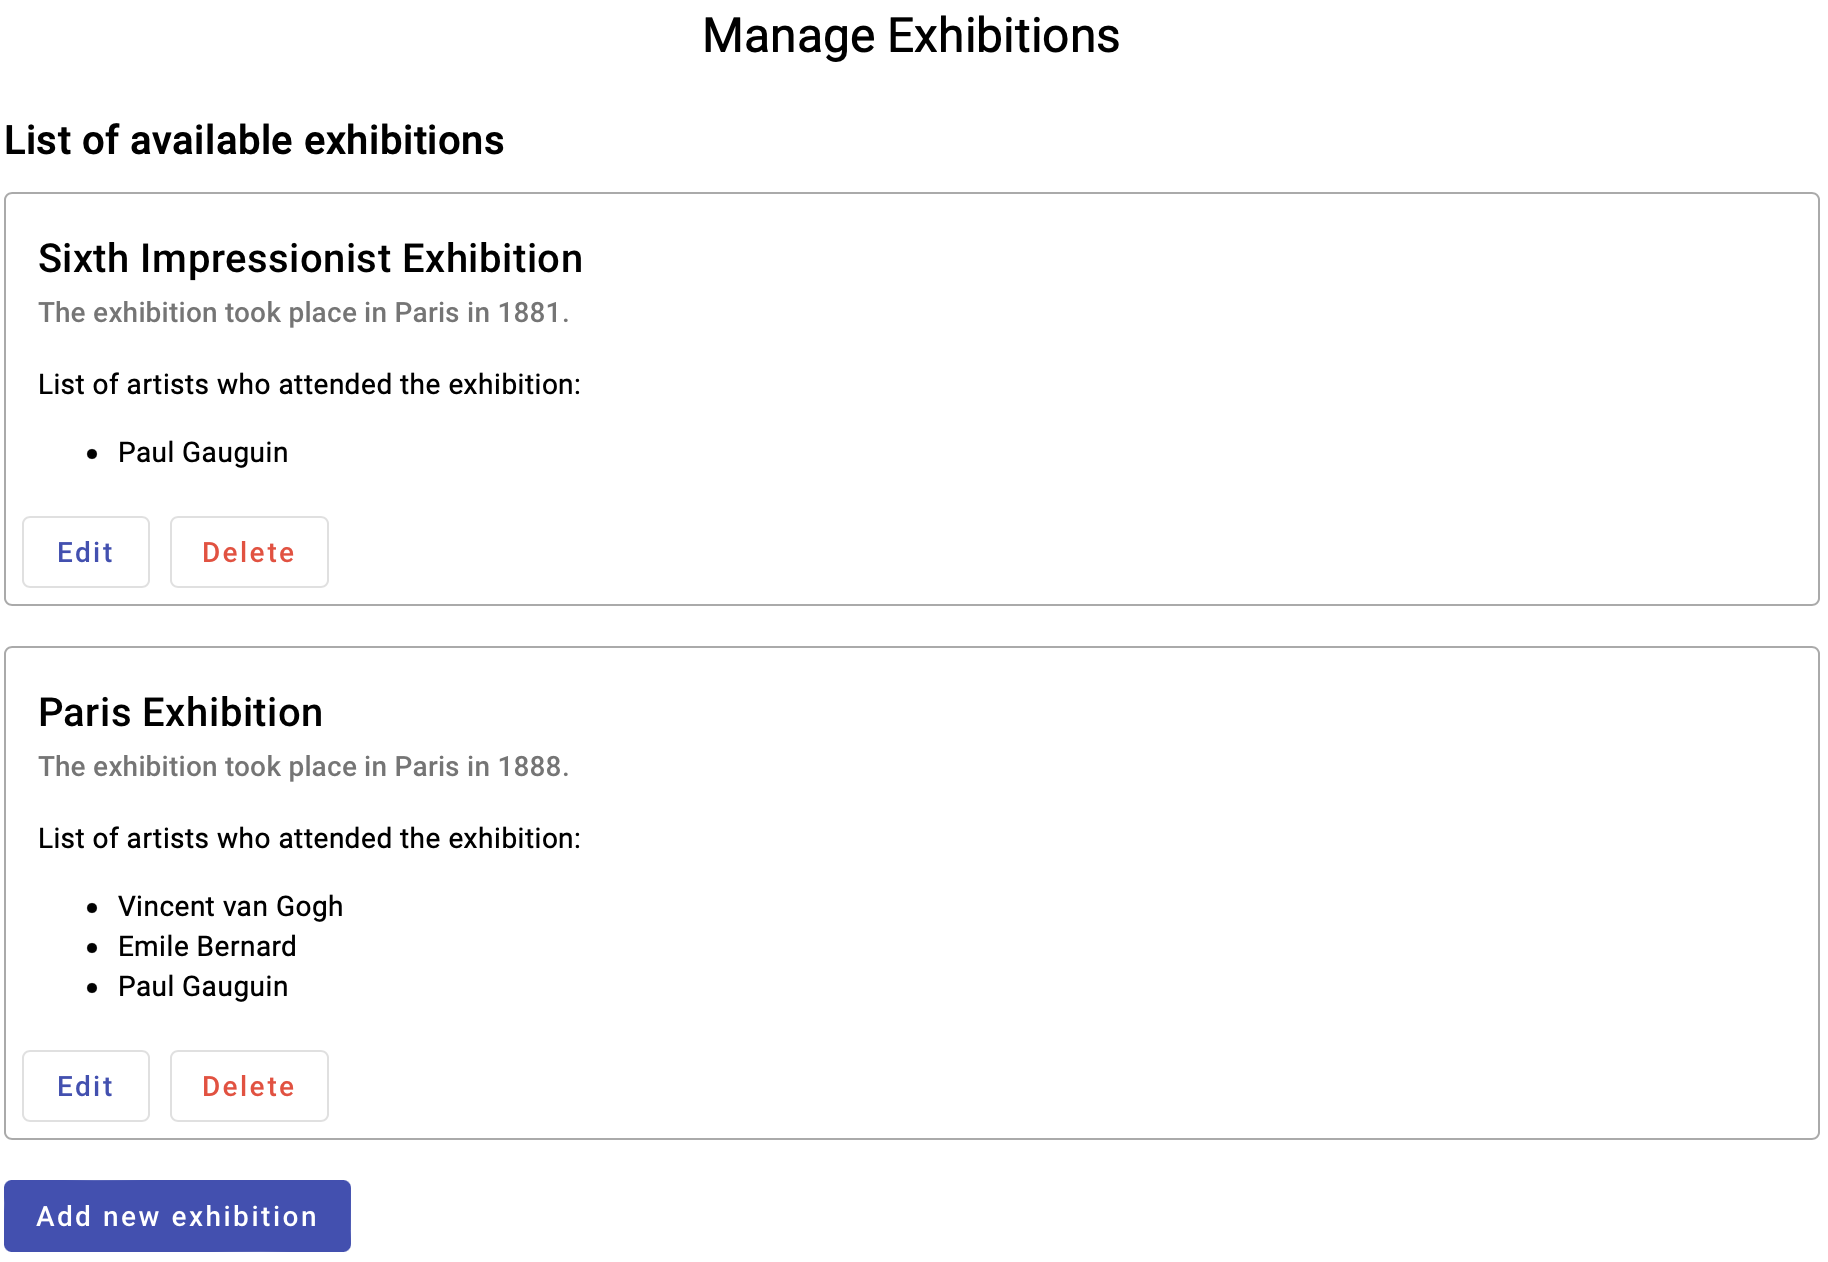
\includegraphics[width=\textwidth]{graphics/3-implementation/5}
    \end{center}
    \caption{Manage exhibitions functionality page}
    \label{fig:figure3.5}
\end{figure}

The main functionality is adding new exhibitions. A dialog is shown with several fields for entering information about the exhibition: the title of
the exhibition, the city it took place in, the start and end date. After entering this information, the user is presented with the list of artists
that lived in the chosen city during the selected time period. In this way, the list of all artists is not given, preventing the user from
selecting any artist that may have not been present at that place during that time. This constraint assures that the list of possible options of
artists that may have attended the exhibition is always accurate.

\clearpage

\begin{figure}[ht!]
    \begin{center}
        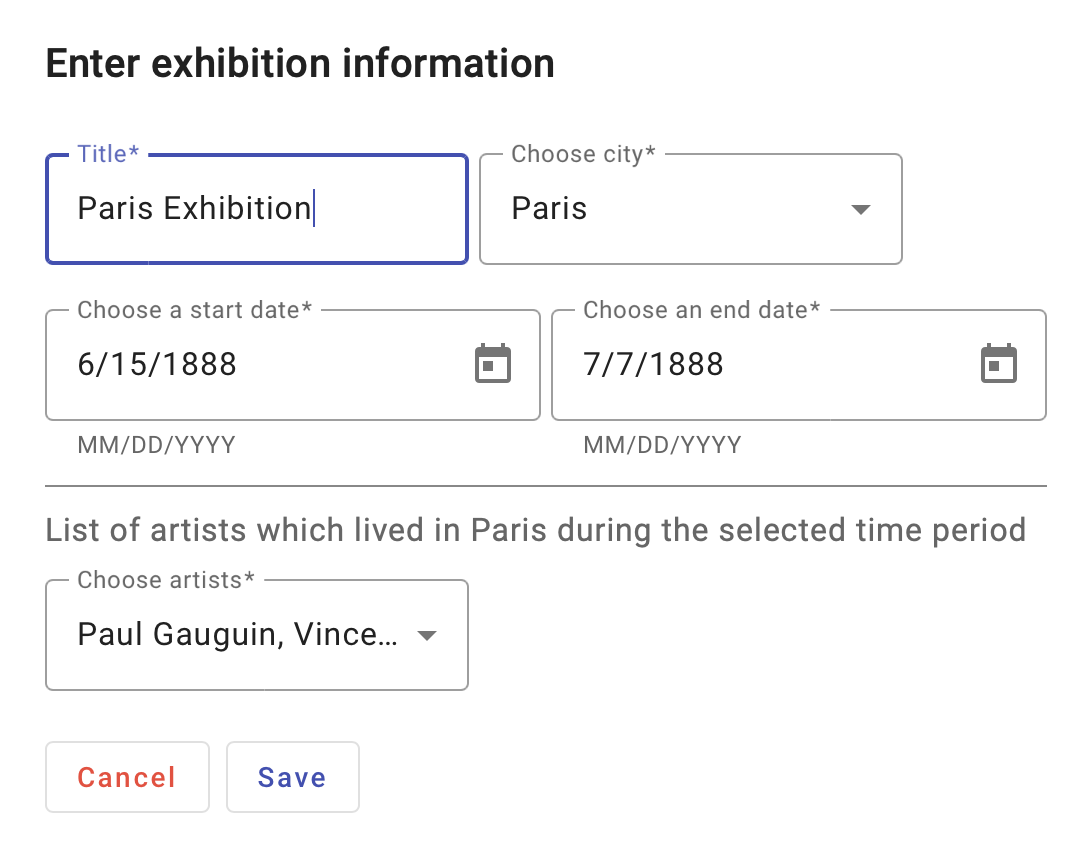
\includegraphics[width=0.7\textwidth]{graphics/3-implementation/6}
    \end{center}
    \caption{Adding a new exhibition dialog}
    \label{fig:figure3.6}
\end{figure}